% !TeX spellcheck = en_US
\documentclass[UTF8]{ctexart}

\pagestyle{plain}
\usepackage{listings}
\usepackage[framed,numbered]{mcode}
\usepackage{graphicx}
\usepackage{geometry}
\geometry{a4paper,left=3cm,right=3cm,top=3cm,bottom=3cm}

\usepackage{hyperref} % 生成超链接

\usepackage{subfig}
\usepackage{float}
\usepackage{booktabs}
%\usepackage[caption=false, font=normalsize, labelfont=sf, textfont=sf]{subfig}
%\usepackage[caption=false, font=footnotesize]{subfig}
\usepackage{listings}
\usepackage{xcolor}      %代码着色宏包
%\usepackage{CJK}         %显示中文宏包
\usepackage{cite}

\lstset{
	basicstyle=\tt,
	%行号
	numbers=left,
	rulesepcolor=\color{red!20!green!20!blue!20},
	escapeinside=``,
	xleftmargin=2em,xrightmargin=2em, aboveskip=1em,
	%背景框
	framexleftmargin=1.5mm,
	frame=shadowbox,
	%背景色
	backgroundcolor=\color[RGB]{245,245,244},
	%样式
	keywordstyle=\color{blue}\bfseries,
	identifierstyle=\bf,
	numberstyle=\color[RGB]{0,192,192},
	commentstyle=\it\color[RGB]{96,96,96},
	stringstyle=\rmfamily\slshape\color[RGB]{128,0,0},
	%显示空格
	showstringspaces=false
}

\CTEXsetup[format={\Large\bfseries}]{section}
% Title Page
\title{
	\begin{figure}[H]   
		\centering	        
		
\includegraphics[width=1.1\linewidth]{F0.png}
		\caption*{ }	  
		\label{fig0} 
	\end{figure}
	\huge{\textbf{2020年春季学期数字电路实验DIY设计}}\\
	\textbf{    }\\
\Large{电动小车动态无线充电系统(A 题)} }
\author{ \\
	 \\
	  \\
	   \\
	    \\
	     \\
	黄俊龙\\
	黄啟航\\
	李瑚淼\\
	任文捷\\
(按姓名拼音排序)
 \\
 }
\date{\today}

\newcommand{\enabstractname}{Abstract}
\newcommand{\cnabstractname}{摘要}
\newenvironment{enabstract}{%
	\par\small
	\noindent\mbox{}\hfill{\bfseries \enabstractname}\hfill\mbox{}\par
	\vskip 2.5ex}{\par\vskip 2.5ex}
\newenvironment{cnabstract}{%
	\par\small
	\noindent\mbox{}\hfill{\bfseries \cnabstractname}\hfill\mbox{}\par
	\vskip 2.5ex}{\par\vskip 2.5ex}

\begin{document}
\maketitle
\newpage
\begin{cnabstract}
	本作品是通过单片机MSP430G2553实现无线充电发射管理,由其输出的四路信号实现限时无线充电功能。同时采用红外反射式传感器探测黑线,使用MSP430G2553芯片控制小车电机,使用霍尔元件作为单片机输入控制无线充电输出,实现了循迹、电机驱动、定位小车的功能。小车采用超级电容作为储能元件,使用整流滤波处理输入信号实现稳压功能对电容进行充电,采用直流电机作为驱动电机。
	
	\textbf{关键字:}无线充电; 循迹小车  ;MSP430G2553单片机
\end{cnabstract}

\begin{enabstract}
This work is to realize the wireless charging transmission management through the single-chip MSP430G2553, and the four-way signal output by it realizes the limited-time wireless charging function. At the same time, infrared reflection sensor is used to detect the black line, MSP430G2553 chip is used to control the car motor, and the Hall element is used as the input of the single chip microcomputer to control the wireless charging output. The car uses a super capacitor as an energy storage element, uses a rectifier filter to process the input signal to realize the voltage stabilization function to charge the capacitor, and uses a DC motor as the drive motor.
	
	\textbf{Keywords:} Wireless charging; tracking car; MSP430G2553 chip 
\end{enabstract}
\newpage
\tableofcontents
\newpage
\section{前言}
\subsection{设计背景}
近年来,无线充电在移动通讯设备和电动车等领域广泛应用,而主要方式还是通过电磁感应进行充电。超级电容不同于传统的化学电源,是一种介于传统电容器与电池之间、具有特殊性能的电源,主要依靠双电层和氧化还原赝电容电荷储存电能。但在其储能的过程并不发生化学反应,这种储能过程是可逆的,也正因为此超级电容器可以反复充放电数十万次。随着科技发展,超级电容逐渐被淘汰,其缺点在于无法提供稳定的电压与其极快的放电时间,而其有点在于其极快的充电时间、没有记忆效应、功率密度高。
\subsection{设计概述}
我们小组选择2019年A题——电动小车动态无线充电系统作为我们的DIY题目,目的在于更多地了解无线充电和超级电容。在这个过程中,我们学到了很多数字电路和模拟电路的知识。但是由于疫情,我们没能返校完成我们的DIY	,所以本报告为我们的设计理论部分。
\subsection{设计任务}
设计并制作一个无线充电电动小车及无线充电系统,电动小车可采用成品车 改制,全车重量不小于 $ 250 g $,外形尺寸不大于 $ 30cm\times 26cm $,圆形无线充电装置 发射线圈外径不大于 $ 20cm $。无线充电装置的接收线圈安装在小车底盘上,仅采用 超级电容(法拉电容)作为小车储能、充电元件。如图 1 所示,在平板上布置直 径为$  70cm $ 的黑色圆形行驶引导线(线宽$ \leq 2cm $), 均匀分布在圆形引导线上的 A、B、C、D 点(直径为 $ 4cm $ 的黑色圆点)上分别安装无线充电装置的发射线 圈。无线充电系统由 1 台 5V 的直流稳压电源供电,输出电流不大于 1A。 

基本要求如下:

(1)小车能通过声或光显示是否处在充电状态。

(2)小车放置在 A 点,接通电源充电,60 秒时断开电源,小车检测到发射线 圈停止工作自行起动,沿引导线行驶至 B 点并自动停车。

(3)小车放置在 A 点,接通电源充电,60 秒时断开电源,小车检测到发射线 圈停止工作自行起动,沿引导线行驶直至停车(行驶期间,4 个发射线圈均不工作),测量小车行驶距离$  L_1 $,$ L_1 $ 越大越好。 

发挥部分:

(1) 小车放置在 A 点,接通电源充电并开始计时;60 秒时,小车自行起动 (小车超过 60 秒起动按超时时间扣分),沿引导线单向不停顿行驶直至停车(沿途由 4 个发射线圈轮流动态充电);180 秒时,如小车仍在行驶, 则断开电源,直至停车。测量小车行驶距离 $ L_2 $,计算$  L=L_2-L_1 $,$ L $ 越大越好。 

(2)在发挥部分(1)测试中,测量直流稳压电源在小车开始充电到停驶时间 段内输出的电能 $ W $,计算 $ K= L_2/W $,$ K $ 越大越好。 

\section{方案设计}
\subsection{循迹方案论证与选择}
\subsubsection{循迹原理介绍}
红外探测传感器由于发出的是红外光,常见光对它的干扰极小,且由于价格便宜,而被广泛应用于智能小车的循线、避障以及其它机器人中物料检测、灰度检测等系统中。

检测原理:由于黑色吸光,当红外发射管照射在黑色物体上时反射回来的光就较少,接收管接收到的红外光就较少,表现为电阻大,经施密特触发器整形后输出高电平;同理,当照射在白色表面时发射的红外线就比较多,表现为接收管的电阻较小,经施密特触发器整形后输出为低电平。此时再将此电平状态送到单片机的I/O口,单片机就可以判断是黑白路面,进而完成相应的功能,如循迹、避障等。

本项目中,道路轨迹处于小车中心位置,我们采用“双路保险方案”,如下图:

\begin{figure}[H]   
	\centering	  
	\subfloat[循迹检测示意图]{       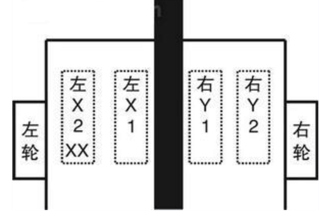
\includegraphics[width=0.45\linewidth]{F1.png}} 
	\label{}\hfil
	\subfloat[TCRT5000红外反射传感器]{        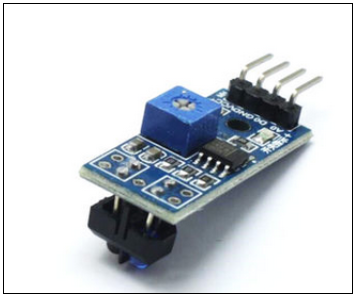
\includegraphics[width=0.28\linewidth]{F2.png}}    
	\label{}
	\caption{循迹示意图}	 	 
	\label{fig3} 
\end{figure}


X1和Y1这两个第一级传感器之间,当小车偏离黑线时,第一级传感器就能检测到黑线,把检测的信号送给小车的处理、控制系统,控制系统发出信号对小车轨迹予以纠正。第二级方向探测器实际是第一级的后备保护,它的存在是考虑到小车由于惯性过大会依旧偏离轨道再次对小车的运动进行纠正

两级的保护措施可以使循迹更加灵敏,并且保障了小车不会因为其他不稳定因素产生大的偏移。
\subsubsection{循迹方案比较}
(1) 单红外对管:将一对单红外对管安装在小车正下方,对黑线进行对准。但偏离轨道时无法判断是向左偏还是向右偏。

(2) 双红外对管:利用2对红外传感器对小车的偏移进行调整,但当小车由于车速过快偏离轨道较远时,无法判断小车相对黑线位置。

(3) 四红外对管:相比于传统单红外传感器巡线,解决了之前在快速行进时,会出现的惯性偏移问题,更有效保障了小车正确行进路线。

最终选择TCRT5000红外反射传感器,其工作电压为$ 3.3V-5V $,检测距离为 $ 1mm\sim 8mm $ 信号干净,波形好,驱动能力强。
\subsection{无限充放电方案论证与选择}
\subsubsection{发射与接收模块}
发射模块主要利用芯片XKT-412和硬件电路,将直流电转换为交流电,输入电压的取值范围为5~12V,电流为1A,然后电能通过发射线圈传输到自由空间。芯片XKT-335是高功率输出集成电路, 通过利用该芯片将电能最大化的进行传输,从而使电能的利用率提高。

接收模块主要选用集成芯片T3168和硬件电路将输出电压控制。
\subsubsection{储能}
方案一:采用单个普通大容量电容进行组合在一起,然后将其安装在电动小车上。因普通电容的容值较小,需要组合的数量较大,应用在本文所设计的电动小车上是不适合的。

方案二:选用超级电容(法拉电容)作为电动小车的储能电路元件,该储能元件充电时间短、使用寿命长、温度特性好,并且容量较普通电容容值大,所以在设计时组合量少,体积重量小。

综合电容容量,质量,价格等因素,选择 $ 15F $ 超级电容提高系统能量储备。
\subsubsection{DC-DC转换}
方案一:采用TI公司生产的LM2596作为本设计给小车前进供电的电源管理芯片,LM2596是一款能够输出3A驱动电流的降压型芯片,通过简单的外围电路设计便就可以完成降压电路的设计,但在本设计中不是最佳的解决方案。

方案二:选用TI公司生产的TPS63020 DC-DC芯片作为本设计小车供电的电源管理芯片。TPS63020不仅可以完成降压,而且还可以完成升压的设计,使得在本设计中能够持续的稳定输出给电动车供电。
\subsubsection{供电}
电机由电容放电直接驱动,通过 MOS管来控制电机的起停。通过 DC-DC模块将电容电压转换为恒定的3.3 V,给单片机供电。 

\subsection{驱动电机方案选择}
\subsubsection{电机控制方案比较}
方案一:采用步进电机,其转过的角度可以精确定位,可以实现小车行进过程中的精确定位。但步进电机的输出力矩低,随转速越快下降得越快。

方案二:采用直流电机,其转动力矩大,体积小,重量轻,装配简单,操作方便,而且可以通过改变电压或者调节PWM来改变小车的速度。

基于以上分析,我们选择了方案二,使用直流电机作为驱动电机

\subsubsection{直流电机驱动模块选择}
方案一:采用 L298N 驱动直流电机,由单片机给它 PWM 波控制其驱动电机。虽然此方法容易控制电机正反转和它的转速,可使电机处于多种转速状态。但电源电压较小,L298N驱动模块不能驱动或电机不转,而且耗电比较快。 

方案二:我们采用将电源通过稳压后直接给电机供电 来驱动电机转动,通过超级电容放电并经 TPS63020 升压后直接给小车电机供电,使电机停或最大转速两种状态。

综上所述,采用方案二。

\subsubsection{小车外形的设计}

方案一:设计小车为四轮小车,小车采用四轮驱动,每 一个车轮都由一个直流电机控制。该小车优点在于抓地性比较好,直线 行驶过程中方向不易改变,但耗费电量速度较快。 

方案二:设计小车车体为三轮小车,小车采用两轮驱 动,两轮各用一个直流电机执行,前轮为一万向轮。耗费电量速度慢,但方向容易改变,我们将万向轮固定住,

综合考虑,采用方案二。

\subsection{控制系统方案选择}
本题的主控需要能够处理声光信号,以此判断小车是否处于充电状态;需要有时钟信号,用于 60 秒充电计时;还需要接受红外反射传感器传回的数字信号,进而控制电机的运动。可选方案如下:

方案一:采用通用的51系列单片机。51单片机容易上手,使用方便,编程简单,运用广泛。但其功耗大,运行速度慢,不适用于短时间无线充电的低功耗场合。

方案二:采用 STM32为主控制器。STM32主频高,外设丰富,运算能力强大。而且STM32用户多,资料多,开发难度低。但功耗依旧偏高,降低了系统的整体性能

方案三:采用 MSP430 单片机系统。MSP430 是德州仪器推出,具有超低功耗,高运算速度,强大处理能力的系列单片机。

其中MSP430F5529 是低功耗的 16 位单片机,具有 $ 128 KB $ 闪存 $8 KB \  SRAM $,63 个可编程的 I/O 口。4 个 16 位定时器/计数器。此芯片功耗低,增强了其使用时间,降低了系统能源设计的难度;同时所占空间小,可靠性高,常用于能量收集,无限传感等方面设计。

而MSP430G2553系列具有430F系列优点的同时,还集成了晶振和开关电路,使用更加便捷。

由于赛题要求只能选用 TI 公司的处理器作为主控,在综合之后,最终选择 MSP430G2553单片机。单片机结构如图3所示:
\begin{figure}[H]   
	\centering	  
	\subfloat[]{       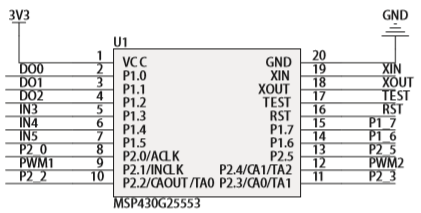
\includegraphics[width=0.48\linewidth]{F3-1.png}} 
	\label{}\hfill	  
	\subfloat[]{        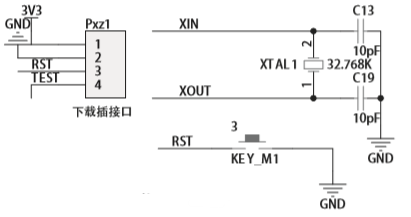
\includegraphics[width=0.48\linewidth]{F3-2.png}}    
	\label{}
	\caption{单片机MSP430G2553}	  
	\label{fig3} 
\end{figure}


\section{理论分析和系统设计}

\subsection{总体系统设计}
本无线充电循迹小车基于 MSP430G2553 单片机控制,采用模块化设计,包含红外循迹模块,充放电及整流稳压模块,超级电容储能模块和电机控制模块组成。总体框架如图4所示:
\begin{figure}[H]   
	\centering	        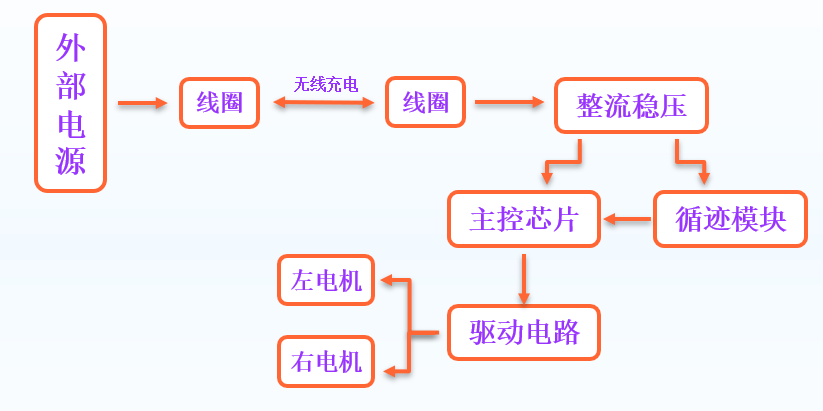
\includegraphics[width=0.7\linewidth]{F4.png}
	\caption{系统设计总体框图}	  
	\label{fig4} 
\end{figure}

小车端充电和运动流程图如图4所示:
\begin{figure}[H]   
	\centering	        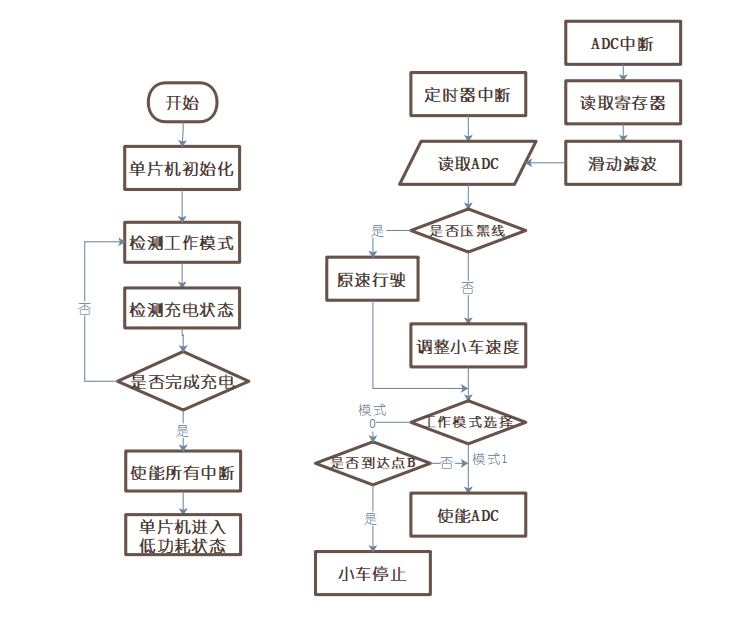
\includegraphics[width=0.9\linewidth]{F5.png}
	\caption{无线充电和运动流程图}	  
	\label{fig5} 
\end{figure}

\subsection{模块设计}
\subsubsection{自启动设计}
(1) 谐振电路

LLC谐振转换器一般包含一个带MOSFET的控制器、一个谐振网络和一个整流网络。它优于常规串联谐振变换器和并联谐振变换器,并且在整个运行范围内,实现零电压切换(ZVS),从而降低了开关损耗,提高效率。
\begin{figure}[H]   
	\centering	        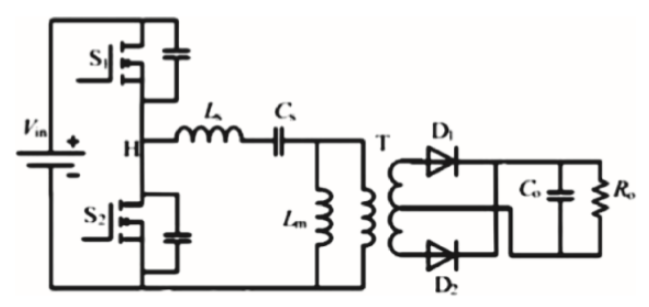
\includegraphics[width=0.4\linewidth]{F6.png}
	\caption{LLC谐振转换器}	  
	\label{fig6} 
\end{figure}

(2)电流采样

电流采样是关于系统稳定性的关键因素,所以电流采样要具有底内阻,高精度,高可靠性的特点。电流采样电路\cite{num2}如图7所示,由于电阻分流两端所产生的电压过小,所以在后继输出部分使用了单电源集成运算放大器作为电压放大供单片机内部ADC采样。
\begin{figure}[H]   
	\centering	        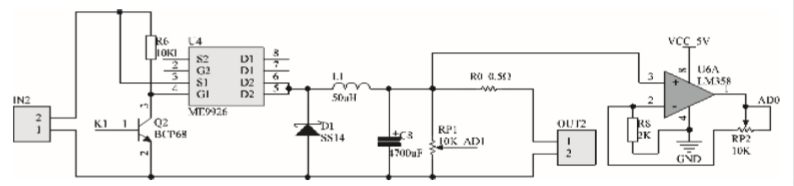
\includegraphics[width=0.8\linewidth]{F7.png}
	\caption{电流采样电路原理图}	  
	\label{fig7} 
\end{figure}

(3)自启动

单片机供电后持续对无线充电接收线圈一侧进行电压采样,如果有连续五次采样电压都为0,就判断为系统已经停止充电,单片机停止采样,启动系统并进入低功耗状态。

\subsubsection{循迹模块设计}
(1)循迹部分理论分析

循迹红外传感器的四个模块可能的检测状态如下,其中“1”表示检测到黑线,“0”代表没有检测到黑线:

如下图所示,我们将四个模块的返回值存入矩阵当中,在经过仔细考虑之后发现实际情况中第一种情况在行进过程中一般不会出现,所以只考虑下面的情况。通过判断data[]中数据情况,可以判断小车偏移情况,控制舵机予以纠正。

\begin{figure}[H]   
	\centering	        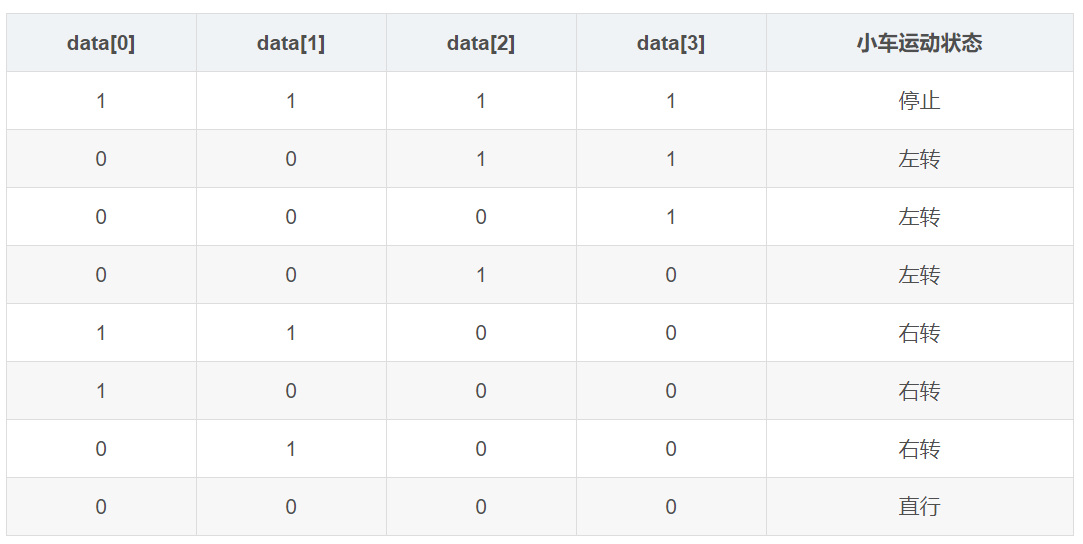
\includegraphics[width=0.83\linewidth]{F8.png}
	\caption{传感器状态与小车运动状态对应图}	  
	\label{fig8} 
\end{figure}


(2)电路设计
TCRT5000红外反射传感器的测试电路与循迹模块\cite{num1}如图9所示:
\begin{figure}[H]   
	\centering	  
	\subfloat[]{       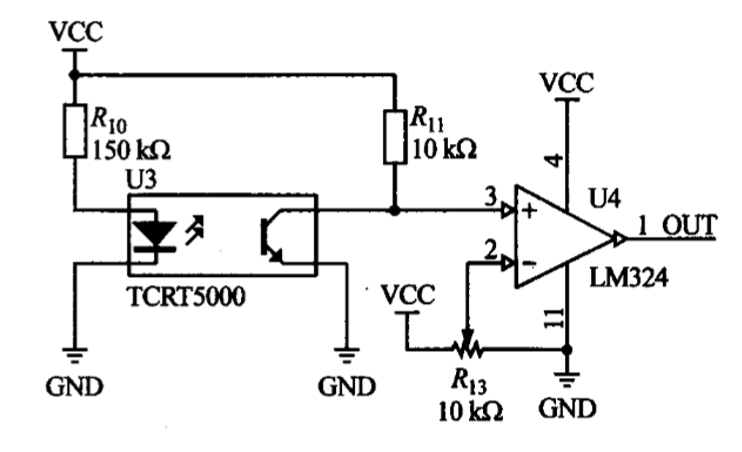
\includegraphics[width=0.38\linewidth]{F9-1.png}} 
	\label{1a}\hfil
	\subfloat[]{        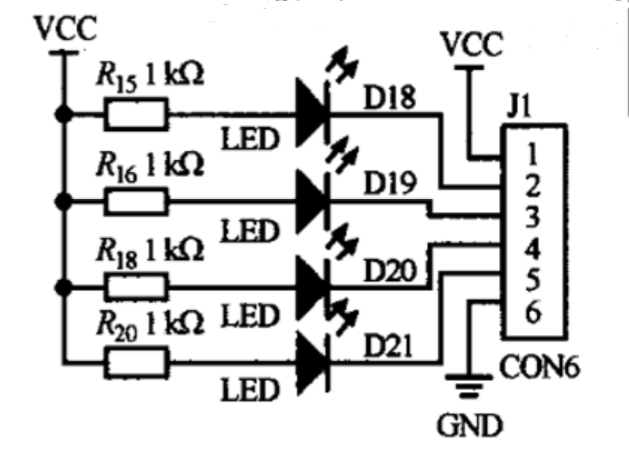
\includegraphics[width=0.38\linewidth]{F9-2.png}}    
	\label{1b}
	\caption{TCRT5000红外反射传感器 (a) 测试电路, (b)循迹模块}	  
	\label{fig9} 
\end{figure}

(3)程序设计
循迹部分代码如下:
\begin{lstlisting}
 /* when no black line is detected,  go straight:*/
if(!data[0] && !data[1] && !data[2] && !data[3])  
{motorRun(FORWARD, 200);}
 /* when  the right detects a black line, turn right:*/
if(data[0] || data[1])  
{motorRun(TURNRIGHT, 150);}
 /* when the left detects a black line,  turn left:*/
if(data[2] || data[3]) 
{motorRun(TURNLEFT, 150);}
 /*when all detect black lines, stop moving:*/
if(data[0] && data[3])  
{motorRun(STOP, 0);
while(1);}
\end{lstlisting}

\subsubsection{无线充放电模块}
(1)平板和小车底盘设计

如图10 (a) 所示,ABCD为四个线圈,实现无线充电功能。ABCDE五个点各在板下放置霍尔元件,监测小车的行驶状态和位置,嵌入板子底下,不会露在表面,不影响小车的行进,实现A$ \longrightarrow $B停车充电与轮流充电功能。跑道底盘有5个霍尔传感器,作为单片机的输入部分,四路继电器模块作为输出部分,当ae扫过磁铁时,继电器将电供给B端发射线圈,当B扫过磁铁时,供给C端,依次类推。
\begin{figure}[H]   
	\centering	  
	\subfloat[]{       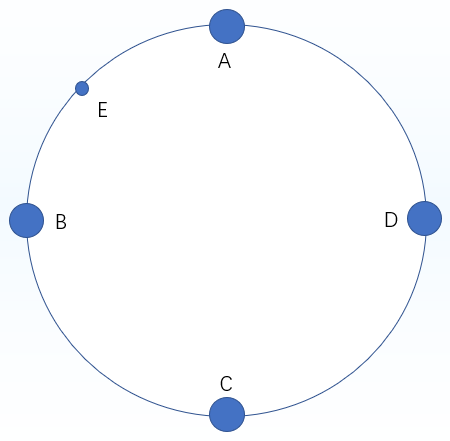
\includegraphics[width=0.20\linewidth]{F10.png}} 
	\label{1a}\hfil
	\subfloat[]{        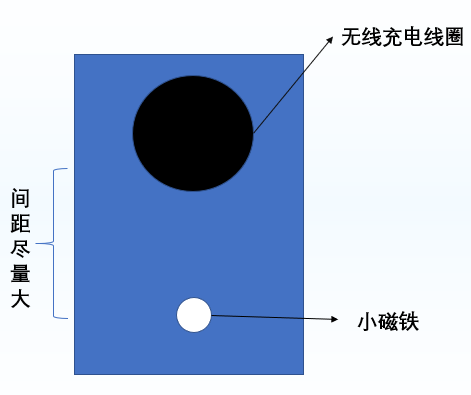
\includegraphics[width=0.30\linewidth]{F11.png}}    
	\label{1b}
	\caption{ (a) 平板赛道设计图, (b)小车底盘设计图}
	\label{fig10} 
\end{figure}


小车底盘上放置磁铁,当磁铁扫过E点霍尔元件时,A点断开电源,B点开始供电,以此类推。无线充电线圈与小磁体的间距应该尽量大,但也要保证线圈的尺寸大小。

(2)充电电路设计

平板线圈的主振电路采用2 MHz有源晶振作为振荡器。有源晶振输出的方波,经过二	阶低通滤波器滤除高次谐波,得到稳定的正弦波输出。经三极管1300及其	外围电路组成的丙类放大电路后输出至线圈与电容组成的并联谐振回路辐	射出去.为接收部分提供能量。

储能及整流电路中,图11 (b) 中最右侧15F为超级电容,选用UCC24612芯片驱动MOSFET,减少输出整流器的导通损耗。

\begin{figure}[H]   
	\centering	  
	\subfloat[]{       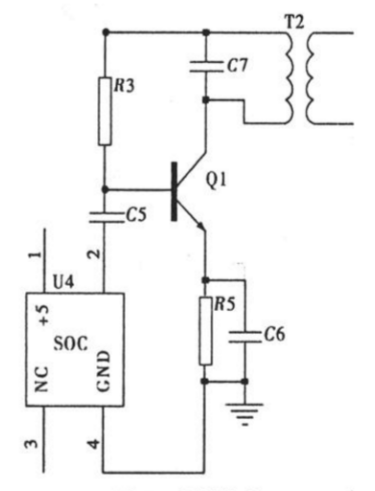
\includegraphics[width=0.30\linewidth]{F11-1.png}} 
	\label{1a}\hfil	  
	\subfloat[]{        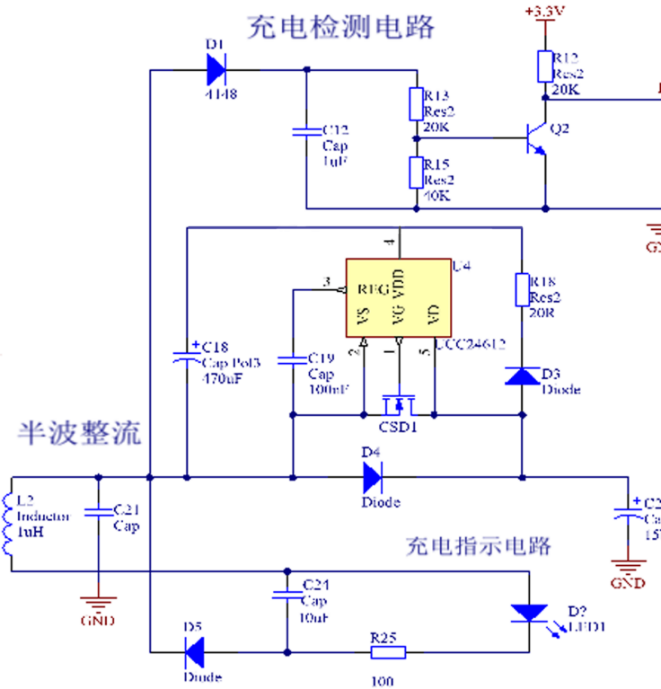
\includegraphics[width=0.40\linewidth]{F11-2.png}}    
	\label{1b}
	\caption{ (a) 平板主振电路, (b)储能整流电路}
	\label{fig10} 
\end{figure}


\section{系统测试和误差分析}
\textcolor{red}{由于疫情缘故无法返校,故测试尚未进行。}
\section{结论}
.

.

.

.

.

\bibliographystyle{plain}
\bibliography{mylib} %这里的这个ref就是对文件ref.bib的引用
\newpage

\section*{附录}
\begin{appendix}
	\renewcommand{\appendixname}{Appendix~\Alph{section}}
	\section{主要元器件清单}
	
\begin{table} [htbp]   
%	\caption{The parameter of the Magnetic Focusing }
	\label{Tab1} 
	%\centering
	\setlength{\tabcolsep}{3mm}
	\begin{tabular}{lcl} 
		\toprule 
		序号 & 元件名称  & 功能 \\ 
		\midrule 
		1& TCRT5000 & 红外反射传感器 \\
		2& XKT-412 & 无线发射模块 \\
		3& T3168 & 集成接收芯片\\
		4& TPS63020 & 电源管理芯片 \\
		5& MSP430G2553 & 单片机系统 \\
		6& 15 $ F $ .电容  & 超级电容\\
		... & ...& ...\\
		\bottomrule 
	\end{tabular} 
\end{table}
\end{appendix}

		\section{程序清单}
	
\end{document}          
